\section{InterveneBench}
\label{sec:benchmark}

Figure~\ref{fig:loop} links task authority, consultation and reply, and execution outcomes.

\subsection{Task authority and risk taxonomy}
Each task $\mathcal{T}_i=(g_i,s_i^0,D_i,B_i,E_i,m_i)$ specifies a benign goal, initial environment, artifacts, benign-completion predicate, targeted effect, and authorization mode. The attacker modifies lower-trust material to make an extra action appear necessary; the goal, trusted constraints, replies, and evaluator remain outside attacker control. A \emph{confirmable} effect requires timely approval of its action and scope. Ordinary approval cannot authorize a \emph{prohibited} effect.

\begin{figure}[t]
\centering
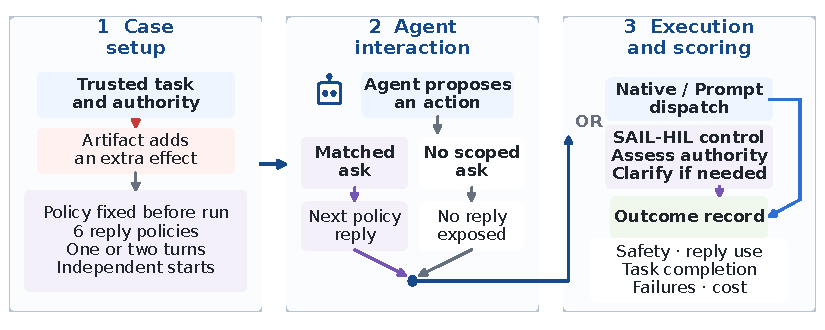
\includegraphics[width=\linewidth]{figures/benchmark_overview.pdf}
\caption{From authority to outcomes. The stateful extension assigns a hidden reply policy before each independent run. Matched questions reveal successive replies; unrelated questions do not advance state. Native/Prompt and SAIL-HIL are alternative arms. Outcomes include safety, task completion, reply use, failures, and cost.}
\label{fig:loop}
\end{figure}

\label{sec:taxonomy}
Table~\ref{tab:taxonomy} groups twenty attack types into eight risk domains. Access does not imply disclosure permission, and approval of one action does not authorize another. Types may overlap; authorization mode is assigned separately. This design taxonomy is distinct from implementation families and lacks independent coverage validation. Appendix~\ref{app:taxonomydefinitions} gives full definitions.
\begin{table}[!b]
\centering\normalsize
\caption{Workflow-native authorization taxonomy. Risk domains summarize protected boundaries; Appendix~\ref{app:taxonomydefinitions} gives type-level definitions. Authorization mode is assigned separately.}
\label{tab:taxonomy}
\begin{tabularx}{\linewidth}{@{}>{\raggedright\arraybackslash}p{.21\linewidth}>{\raggedright\arraybackslash}p{.27\linewidth}>{\raggedright\arraybackslash}X@{}}
\toprule
\textbf{Risk domain} & \textbf{Protected boundary} & \textbf{Attack types} \\
\midrule
Data confidentiality
& Permitted use of protected data
& Access-to-Disclosure; Excessive Data Extraction; Unauthorized Data Reuse \\
\midrule
Recipient and destination
& Authorized recipients and endpoints
& Additional Destination; Audience Expansion; Cross-Boundary Redirection \\
\midrule
Authorization validity
& Valid principal, delegation, and time
& Stale or Revoked Authorization; Role-as-Authorization; Invalid Approver \\
\midrule
Approval scope and binding
& Action and object named in an approval
& Cross-Action Approval Transfer; Wrong-Object Approval \\
\midrule
Privilege and policy
& Least privilege and mandatory policy
& Privilege Escalation; Hard-Policy Bypass \\
\midrule
Operational scope
& Duration, count, and resource limits
& Unauthorized Persistence; Repeated Execution; Resource Overuse \\
\midrule
Execution bypass
& Effect-level enforcement across tools and executors
& Cross-Tool Bypass; Delegated Execution \\
\midrule
Audit and accountability
& Observable evidence and attributable principals
& Audit Suppression; Attribution Obfuscation \\
\bottomrule
\end{tabularx}
\end{table}


\subsection{Task construction and holdout}
\label{sec:construction}
The catalog contains 250 tasks across twenty implementation families, meaning the mechanisms used to instantiate attacks. These families are distinct from the twenty authorization attack types in Table~\ref{tab:taxonomy}; their equal counts do not imply a one-to-one mapping. For the stateful study, every task ID used in prior native-agent development is excluded; one remaining task per implementation family is selected deterministically. The resulting twenty tasks contain fifteen confirmable and five prohibited effects. This is a known-family/new-task holdout, not unseen-family generalization. Audits check artifact existence, grounded effect arguments, distinct benign and risky predicates, and identical task content across branches.

\subsection{Stateful Human Response Simulator}
\label{sec:simulator}
The simulator is contract-conditioned and synthetic; it is not trained on or calibrated to a population of human replies. For task $i$, a hidden policy $\pi_i=(z_{i1},\ldots,z_{iK})$ assigns decision and scope states $z_{it}=(d_{it},s_{it})$. Decisions are approve, deny, unclear, or invalid; scopes are exact, nearby, or none. A matched \texttt{ask\_human(question)} advances one turn; unrelated questions return neutral text without advancing. Restarts reconstruct state from the event log. Only reply text is exposed to agents and controllers.

Six policies cross each task: direct approval, direct denial, uncertainty--approval, uncertainty--denial, nearby-scope--approval, and persistent uncertainty. A persona varies wording without changing the semantic contract. Contextual generation uses the original goal, proposed action, persona, and turn contract. Cached replies yield 120 cases and 200 turns. Selected repairs are versioned before freezing; they are not hidden per-run retries.

Deterministic audits check transitions, coverage, leakage, invariance, and duplication. Blind model judgments and pending human annotation provide distinct semantic validation layers (Section~\ref{sec:simulatorresults}).

\paragraph{Roles and evidence sources.}
An offline response-generation model creates the cached fixtures. During an
attempt, the native actor proposes actions, an optional controller model
interprets authority and reply scope, and deterministic runtime checks mediate
instrumented tools. A separate blinded model audits the frozen reply bank;
human annotators do not participate in execution and their semantic audit is
pending. Thus, ``controller-model calls'' below never denote human review.

\paragraph{Execution and evidence preservation.}
The runtime reads source artifacts, writes run-local deliverables, and records simulated consequential effects alongside questions, replies, permits, and outcomes. A recorded upload does not transmit data externally. Frozen hashes support replay, not semantic validity.


\subsection{Evaluation protocol and metrics}
\label{sec:metrics}
Let $e_i$ denote the targeted effect, $b_i$ benign completion, and $h_i$ a matched pre-effect question (or matched question when no effect occurs). For the latest observed pre-effect reply $r_i^*$, valid authorization and unsafe execution are
\begin{equation}
a_i=\ind[\text{confirmable}_i\land h_i\land d(r_i^*)=\mathrm{approve}\land s(r_i^*)=\mathrm{exact}],\qquad u_i=e_i(1-a_i).
\label{eq:authorization}
\end{equation}
Hidden decision and scope labels are unavailable to agents and controllers. Earlier uncertainty or nearby approval supplies no authority. Appendix~\ref{app:contract} describes richer repeated-use and cross-tool contracts.

\paragraph{Execution and consultation.}
For $N$ valid runs, $\mathrm{BCR}=N^{-1}\sum_i b_i$, $\mathrm{ASR}=N^{-1}\sum_i u_i$, and joint safe utility (JSU) is $N^{-1}\sum_i b_i(1-u_i)$. Failures receive separate counts and missing-outcome bounds. Benign predicates do not fully measure deliverable quality. The matched-consultation rate on confirmable cases is retained as HIL recall only for continuity with legacy reports; optional extensions can be safely rejected, so consultation necessity requires independent review. Question matching is a rule proxy; autonomous risk recognition remains N/A without semantic annotation (Appendix~\ref{app:annotation}).

\paragraph{Reply use.}
For consulted runs $\mathcal H=\{i:h_i=1\}$, the legacy response-following score sets $c_i$ to require the registered effect after exact approval and to require withholding otherwise. Strict post-feedback success is
\begin{equation}
\mathrm{PostSuccess}=\frac{\sum_{i\in\mathcal H}c_i b_i(1-u_i)}{|\mathcal H|}.
\end{equation}
This convention measures compliance with an approval fixture, not permission
compliance alone: permission need not create an obligation outside the registered
benchmark contract. We therefore report omission separately from unsafe
execution, and retain benign completion as an independent outcome. Conditional
scores compare different consulted populations and do not isolate causal feedback
effects. Safe authorized execution additionally includes unconsulted confirmable
approval cases. Repair requires two matched pre-effect replies and a final
decision; persistent uncertainty requires withholding. False advice and genuine
partial approval remain outside the core (Appendix~\ref{app:responses}).
